%%%%%
% ch5 %
%%%%%

\chapter{Forced and natural convection}
\section{Conduction and convection}
	\begin{wrapfigure}[10]{l}{4cm}
	\vspace{-5mm}
	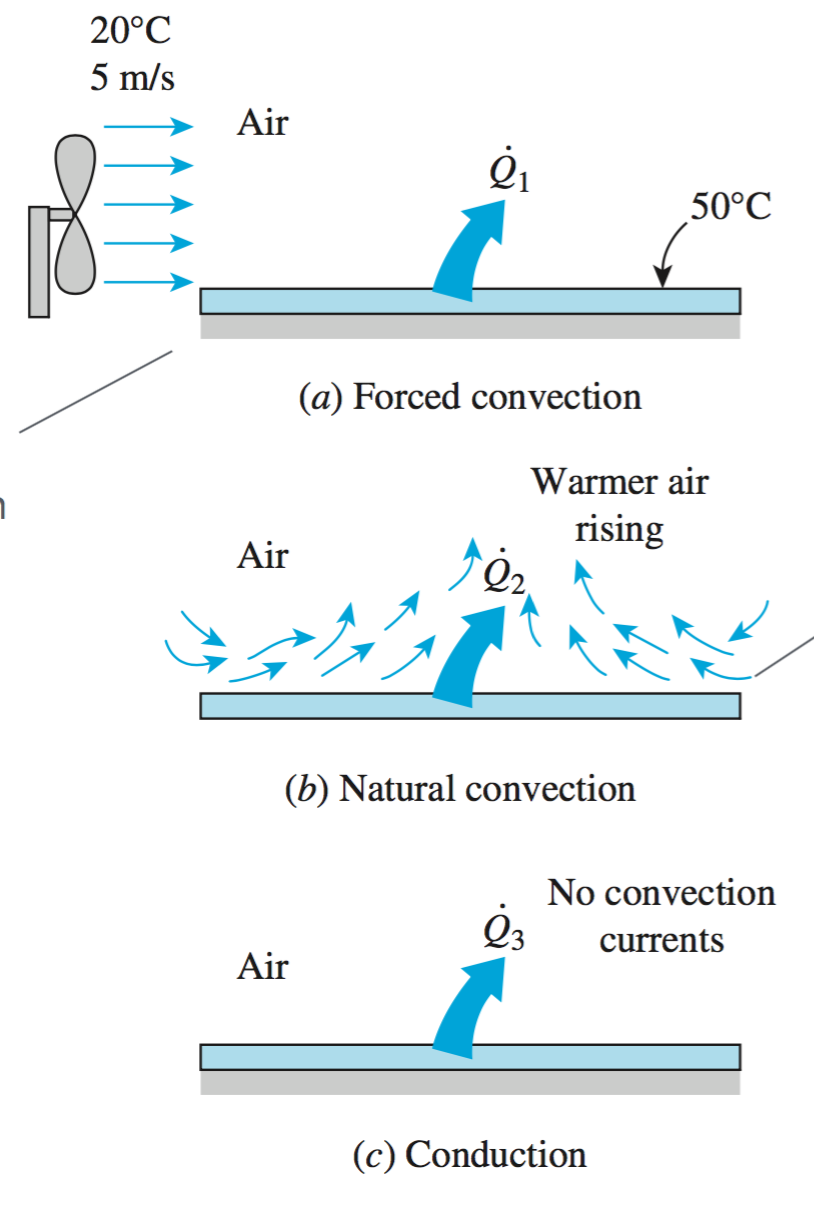
\includegraphics[scale=0.25]{ch5/1}
	\end{wrapfigure}	
	Heat transfer through a solid is always conduction, the molecules position are relatively fixed. Heat transfer in a liquid or gas is convection if there is a \textbf{bulk} fluid motion and is conduction when there isn't. Conduction in a fluid is the limiting case of convection where the fluid is \textbf{quiescient}\footnote{Au repos}.  \\
	Convection is complicated due to the fact that it involves fluid motion as well as conduction. Fluid motion \textbf{enhances}\footnote{Améliore} fluid motion, it brings the cooler and warmer part of fluid into contact, increasing the rate of heat transfer. \\
	Natural convection is caused by a density gradient. 

\section{Macroscopic energy balance}
	\begin{wrapfigure}[6]{r}{5cm}
	\vspace{-5mm}
	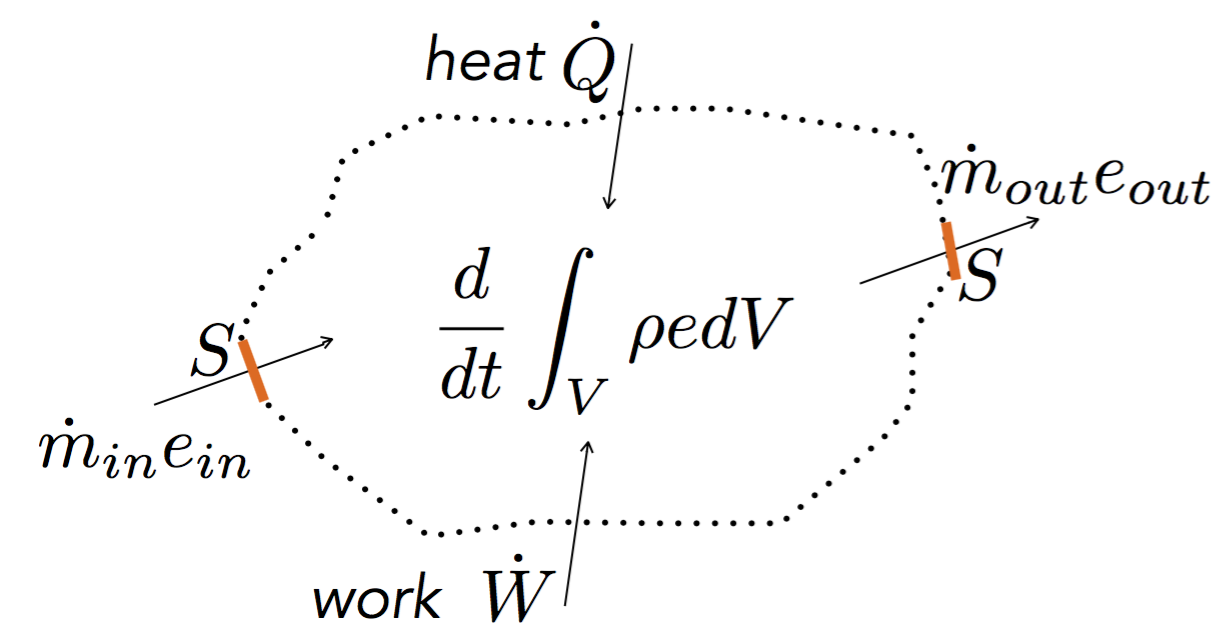
\includegraphics[scale=0.25]{ch5/2}
	\end{wrapfigure}	
	Let's consider a control volume and let's apply an energy balance, using $e = u + \frac{v^2}{2} + gz$ where the first term is the internal energy, the second the kinetic energy and the last the potential energy 
	\begin{equation}
		\frac{d}{dt}\int _V \rho e \, dV = (\rho v e S)_{in} - (\rho v e S)_{out} + \dot{W} + \dot{Q}
	\end{equation}
	Where the work can be decomposed in a \textbf{boundary} and a \textbf{useful} work and the heat is given by
	\begin{equation}
		\dot{W} = \dot{W}_f + \dot{W}_p = pvS + \dot{m}w_p = \dot{m}\left( \frac{p}{\rho}+w_p \right) \qquad and \qquad \dot{Q} = \dot{m} q
	\end{equation}		 
	The transient form is given by 
	\begin{equation}
		\frac{d}{dt}\int _V \rho e \, dV = - \Delta (\frac{1}{2}\rho v^3S) - g \Delta (\rho v z S) - \Delta (pvS) - \Delta (\dot{m}u) + \dot{m}w_p + \dot{m}q
	\end{equation}
	The steady form 
	\begin{equation}
		0 = \Delta \left( \frac{1}{2}v^2 + gz + u + \frac{p}{\rho} \right) - q - w_p 
	\end{equation}
	
	\subsection{Relation with the generalized Bernouilli equation}
		